\chapter{BIBLIOTECAS DE VISÃO COMPUTACIONAL}

No mercado de software atual, existem bibliotecas que auxiliam o desenvolvimento de sistemas de Visão Computacional, direcionadas em diversos focos. Muitas dessas ferramentas têm como objetivo suportar questões específicas do campo de estudo de Visão Computacional.

Apesar de não ser o foco deste trabalho, algumas dessas bibliotecas merecem destaque. Uma delas se trata do VLFeat\footnote{\url{http://github.com/mmmikael/vlfeat}}, biblioteca que possui em sua implementação algoritmos populares de Visão Computacional. Outra biblioteca a ser destacada é o VIGRA\footnote{\url{http://hci.iwr.uni-heidelberg.de/vigra}}, que enfatiza o uso de algoritmos flexivéis, construídos usando programação genérica \cite{MUSSER}.

Outras bibliotecas por sua vez possuem recursos que ampliam seu uso em diversas áreas no desenvolvimeto de sistemas de Visão Computacional. Essas bibliotecas são suportadas por diversas linguagens, tanto de baixo nível como de alto nível. Visando a boa produtividade e simples manuseio, optou-se pela abordagem de linguagens de programação de alto nível. Por se tratar de uma linguagem de simples utilização e aprendizado, foi escolhida a linguagem de programação Python neste trabalho. Essa linguagem conta com diversos recursos de uso simples e possui boa integração com as bibliotecas mais utilizadas na área de Visão Computacional.

No grupo de bibliotecas suportadas pela linguagem Python, a que mais se destaca é o OpenCV. Através do uso de interfaces, a utilização da ferramenta tem facilitado o desenvolvimento de aplicações de Visão Computacional, além de permitir o melhor entendimento da área. Existe também o \textit{framework} SimpleCV, com a missão de simplificar ainda mais o uso das interfaces do OpenCV para Python.

Neste Capítulo, são mostradas a utilização e instalação dessas ferramentas de uso geral para o desenvolvimento de sistemas de Visão Computacional suportadas pela linguagem Python.

\section{OpenCV}

Considerada como uma das mais completas bibliotecas na área de Visão Computacional \cite{THORNE} \cite{SEYDOUX}, o OpenCV\footnote{\url{http://opencv.willowgarage.com}} se destaca pelo seu uso abrangente, possuindo mais de 500 funções que implementam técnicas em diversas áreas de Visão Computacional. Dentre as áreas que a biblioteca atua estão: Processamento de Imagem, Segmentação, Transformação, Rastreamento, Calibração de Câmera, entre outras.

Desenvolvida pela Intel, a biblioteca do OpenCV foi criada para prover uma infraestrutura para criação rápida de aplicações de Visão Computacional. Por possuir o foco em aplicações em tempo real, seu código é escrito na linguagem C e C++. Essas linguagens são mais próximas das linguagens de máquina, desta forma, tendem a ter um desempenho superior às linguagens mais atuais, que necessitam ser interpretadas por uma máquina virtual. A utilização do OpenCV pode ainda ser flexibilizada através de interfaces, criadas para se comunicar com outras linguagens de programação como Java, Python e Ruby.

O uso do OpenCV pode ser otimizado com a utilização da biblioteca proprietária \textit{multi-core ready} IPP (\textit{Integrated Performance Primitives}), que possui funções altamente otimizadas para multimídia, processamento de dados e aplicações de comunicação \cite{IPP}. Em estudos realizados por \citeonline{BRADSKI}, a biblioteca é comparada trabalhando de forma independente e integrada com a biblioteca IPP. Essa comparação é apresentada na Figura \ref{img:comparativo}, onde é possível observar o ganho razoável de performance da biblioteca ao ser utilizada em conjunto com a IPP.

\begin{figure}[H]
    \centering
    {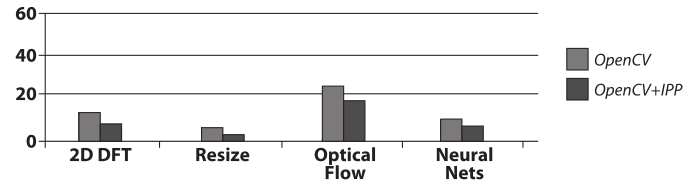
\includegraphics[scale=0.5]{figuras/comparativo}}
    \caption{Comparativo de desempenho entre a ferramenta OpenCV com e sem a biblioteca proprietária da Intel. Adaptado de \cite{BRADSKI}.}
    \label{img:comparativo}
\end{figure}

\subsection{Estrutura}

Baseando-se em relatos de \citeonline{BRADSKI}, o OpenCV é estruturado em cinco componentes principais. As partes de mais alto nível são dividias em: \textit{CV}, \textit{MLL} e \textit{HighGUI}. Como é possível ver na Figura \ref{img:estrutura_opencv}, no componente \textit{CV} está toda a parte de Processamento de Imagem e algoritmos de Visão Computacional. O componente \textit{MLL} contém ferramentas de \textit{clustering} e métodos de classificadores estatísticos. A parte de \textit{HighGUI}, como o nome sugere, contém componentes de interface com usuário, assim como rotinas de entrada e saída de vídeos e imagens. Da mesma forma, no \textit{CXCORE} estão contidas todas as estruturas de dados usadas no OpenCV. Nesse componente também existem algoritmos para manipulação de arquivos XML, sendo possível realizar leitura e gravação de dados. Outro recurso reunido nesse componente bastante utilizado pelos desenvolvedores são as funções de desenho. Através delas, é possível, por exemplo, destacar em uma imagem ou vídeo uma região de interesse (ROI).

Além dos componentes descritos, o OpenCV ainda conta com um componente auxiliar, nomeado de \textit{CvAux}, contendo métodos experimentais. A ideia desse módulo é conter funções de Visão Computacional em fases de testes que podem ser usadas pelos desenvolvedores, e com a aceitação ou não de cada função, a mesma é inserida nos módulos principais como uma função oficial do OpenCV.

\begin{figure}[h]
    \centering
    {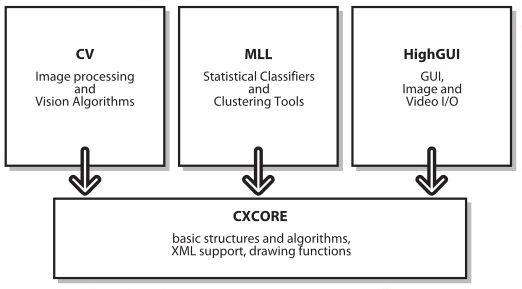
\includegraphics[scale=0.75]{figuras/estrutura_opencv}}
    \caption{Estrutura da biblioteca OpenCV \cite{BRADSKI}.}
    \label{img:estrutura_opencv}
\end{figure}

Como interfaces do OpenCV para linguagem Python, existem duas que cumprem esse papel. A primeira, declarada como \textit{cv2.cv}, é uma implementação mais antiga e trabalha com classes da própria interface. A segunda, nomeada como \textit{cv2}, possui mais dinamicidade em seu uso, permitindo atribuições a tipos de dados nativos do Python. Exemplificando a comparação das duas interfaces, ao carregar uma imagem em ambas, observa-se a diferença em como cada uma delas trata os dados (Código \ref{code:cv_e_cv2}).

\begin{code}{python}{O tipo das variáveis se diferem devido o uso de \textit{bindings} diferentes.}{code:cv_e_cv2}
In [1]: img = cv.LoadImage('logo_iff.png')
In [2]: img
Out[2]: <iplimage(nChannels=3 width=291 height=385 widthStep=876 )>

In [3]: img2 = cv2.imread('logo_iff.png')
In [4]: img2
Out[4]: array([[[255, 255, 255],...,[255, 255, 255]]], dtype=uint8)

In [5]: type(img2)
Out[5]: <type 'numpy.ndarray'>
\end{code}

\subsection{Instalação}
\label{section:install_opencv}

Nas pesquisas realizadas, foi utilizado o sistema operacional Ubuntu em sua versão 11.10, em conjunto da biblioteca OpenCV em sua versão 2.4.2 e a linguagem de programação Python em sua versão 3.0. Buscando uma instalação mais completa e com a maioria dos recursos disponíveis, procurou-se reunir a maior parte das dependências da ferramenta. Contudo, não foi possível realizar a instalação da biblioteca IPP, por se tratar de uma biblioteca proprietária.

Antes de iniciar a instalação do OpenCV, recomenda-se a remoção das bibliotecas usadas pela ferramenta que já estejam instaladas no sistema operacional \cite{ERALP}. O Código \ref{code:remover_pacotes_padrao} apresenta a remoção das bibliotecas comumente encontradas no sistema operacional Linux Ubuntu 11.10.

\begin{terminal}{Remoção de pacotes instalados por padrão no sistema operacional Linux Ubuntu 11.10.}{code:remover_pacotes_padrao}
sudo apt-get remove ffmpeg x264 libx264-dev
\end{terminal}

Para a instalação da biblioteca, é necessário baixar o pacote compactado em sua página oficial. A versão usada no trabalho foi a 2.4.2. A instalação da biblioteca é realizada através de uma ferramenta de construção de sistemas, o CMake (Código \ref{code:install_cmake}). Além disso, existem outras dependências que precisam ser instaladas antes da execução da instalação do OpenCV (Código \ref{code:install_dependencias}).

\begin{terminal}{Instalação da ferramenta CMake.}{code:install_cmake}
sudo apt-get install cmake
\end{terminal}

\begin{terminal}{Instalação de dependências do OpenCV.}{code:install_dependencias}
sudo apt-get install build-essential
sudo apt-get install python-dev python-numpy python-sphinx
sudo apt-get install libgtk2.0-0 libgtk2.0-dev
sudo apt-get install libjpeg8 libjpeg8-dev
sudo apt-get install libgstreamer0.10-0 libgstreamer0.10-dev gstreamer0.10-tools \
  gstreamer0.10-plugins-base libgstreamer-plugins-base0.10-dev \
  gstreamer0.10-plugins-good gstreamer0.10-plugins-ugly gstreamer0.10-plugins-bad \
  gstreamer0.10-ffmpeg
sudo apt-get install libjasper-dev
sudo apt-get install libavcodec-dev
sudo apt-get install libdc1394-22-dev
sudo apt-get install libavformat-dev
sudo apt-get install libv4l-dev
sudo apt-get install libswscale-dev
\end{terminal}

O FFmpeg, conjunto de ferramentas para gravação, conversão e criação de stream de áudio e vídeo, uma das dependências do OpenCV, necessita da instalação prévia de outras bibliotecas para seu funcionamento. Essas dependências são descritas no Código \ref{code:dependencias_ffmpeg}. Após a instalação destas dependências, instala-se o FFmpeg (Código \ref{code:install_ffmpeg}).

\begin{terminal}{Instalação das dependências do FFmpeg.}{code:dependencias_ffmpeg}
sudo apt-get install libfaac-dev libjack-jackd2-dev libmp3lame-dev \
  libopencore-amrnb-dev libopencore-amrwb-dev libsdl1.2-dev libtheora-dev \
  libva-dev libvdpau-dev libvorbis-dev libx11-dev libxfixes-dev libxvidcore-dev \
  texi2html yasm zlib1g-dev libx264-dev
mkdir ~/src
cd ~/src
wget ftp://ftp.videolan.org/pub/videolan/x264/snapshots/ \
	x264-snapshot-20120820-2245-stable.tar.bz2
tar xvf x264-snapshot-20120820-2245-stable.tar.bz2
cd x264-snapshot-20120820-2245-stable/
./configure --enable-static
make
sudo make install
\end{terminal}

\begin{terminal}{Instalação do FFmpeg.}{code:install_ffmpeg}
cd ~/src
wget http://ffmpeg.org/releases/ffmpeg-0.11.tar.bz2
tar xvf ffmpeg-0.11.tar.bz2
cd ffmpeg-0.11
./configure --enable-gpl --enable-libfaac --enable-libmp3lame \
  --enable-libopencore-amrnb --enable-libopencore-amrwb --enable-libtheora \
  --enable-libvorbis --enable-libx264 --enable-libxvid --enable-nonfree \
  --enable-postproc --enable-version3 --enable-x11grab
make
sudo make install
\end{terminal}

Outra dependência do OpenCV é a biblioteca V4L, uma interface de captura de vídeo para programação de aplicativos para Linux. Pode ser baixada e instalada através dos comandos mostrados no Código \ref{code:install_v4l}.

\begin{terminal}{Instalação do V4L.}{code:install_v4l}
cd ~/src
wget http://www.linuxtv.org/downloads/v4l-utils/v4l-utils-0.8.8.tar.bz2
tar xvf v4l-utils-0.8.8.tar.bz2
cd v4l-utils-0.8.8
make
sudo make install
\end{terminal}

Agora é possível executar a instalação do OpenCV. Após realizada a descompactação do pacote, na pasta do OpenCV, crie um diretório onde estarão contidos os arquivos (Código \ref{code:install_opencv1}).

\begin{terminal}{Comandos iniciais para instalação do OpenCV.}{code:install_opencv1}
mkdir release
cd release
\end{terminal}

O comando \textit{cmake} irá construir os executáveis da instalação do OpenCV (Código \ref{code:install_opencv2}).

\begin{terminal}{Execução da instalação do OpenCV através do CMake.}{code:install_opencv2}
cmake -D CMAKE_BUILD_TYPE=RELEASE -D CMAKE_INSTALL_PREFIX=/usr/local \
  -D BUILD_NEW_PYTHON_SUPPORT=ON -D BUILD_EXAMPLES=ON ..
\end{terminal}

Ao executar o comando acima, é possível visualizar quais depedências foram reconhecidas. No geral, as mais importantes são: GTK+ 2.x, FFMPEG, GStreamer e V4L/V4L2. Por fim, é necessário executar os comandos que irão de fato instalar a biblioteca na máquina (Código \ref{code:install_opencv3}).

\begin{terminal}{Comandos finais para instalação do OpenCV.}{code:install_opencv3}
make
sudo make install
\end{terminal}

\subsection{Uso prático}

O OpenCV conta com diversos exemplos em várias linguagens em seu subdiretório (\textit{OpenCV-2.4.2/samples}). Sua documentação também é bastante rica, e pode ser acessada através de seu site\footnote{\url{http://opencv.itseez.com}}, contendo descrição e exemplos dos recursos da biblioteca.

Tomando como base esse material, foi selecionado um conjunto expressivo de comandos da biblioteca, para que seja possível uma rápida familiarização com a ferramenta. Começando com um exemplo básico, é possível carregar e mostrar uma imagem na tela através dos comandos do Código \ref{code:opencv_imread}.

\begin{code}{python}{Carregamento básico de imagem utilizando OpenCV.}{code:opencv_imread}
import cv2
img = cv2.imread('caminho_da_imagem')
cv2.imshow('titulo', img)
cv2.waitKey(0)
\end{code}

A primeira linha importa a interface do OpenCV, que no caso é a \textit{cv2}. Caso seja necessário o uso da interface alternativa, basta substituir \textit{cv2} por \textit{cv2.cv}. O Código \ref{code:opencv_print_img} mostra o conteúdo do \textit{array} da imagem carregada, com os valores RGB de cada \textit{pixel}.

\begin{code}{python}{Comando para visualização dos valores atribuidos a variável \textit{img}.}{code:opencv_print_img}
print img
\end{code}

A saída será um \textit{array} (Código \ref{code:saida_array}), onde para cada grupo de valores RGB é montado um \textit{array}, que por sua vez é agrupado e compõe uma linha vertical da imagem. Então cada \textit{array} é agrupado e assim se forma um \textit{array} que representa por completo a imagem carregada. Dessa forma, se torna flexível a realização de diferentes tipos de operações, como recortar e converter tipos (Código \ref{code:array_oper}).

\begin{code}{python}{Saída do \textit{array}, representando uma imagem carregada pela interface cv2.}{code:saida_array}
[[[255 255 255]
  [255 255 255]
  [255 255 255]
  ...,
  [255 255 255]
  [255 255 255]
  [255 255 255]]
 ...,
 [[255 255 255]
  [255 255 255]
  [255 255 255]
  ...,
  [255 255 255]
  [255 255 255]
  [255 255 255]]]
\end{code}

\begin{code}{python}{Recorte na imagem pode ser realizado através de manipulações com \textit{arrays}.}{code:array_oper}
parte_um = img[:len(img)/2]
parte_dois = img[len(img)/2:]
\end{code}

Pelo fato da variável \textit{img} ser de um tipo conhecido pela linguagem Python, as manipulações com seus valores se tornam simples. Para salvar as variáveis, cada uma contendo metade da imagem, utiliza-se o que é exposto no Código \ref{code:save_imgs}.

\begin{code}{python}{Imagens são salvas utilizando o método do OpenCV que realiza essa operação.}{code:save_imgs}
cv2.imwrite('DIR_PROJETO/images/img1.jpg', parte_um)
cv2.imwrite('DIR_PROJETO/images/img2.jpg', parte_dois)
\end{code}

Quanto as conversões de espaço de cor, a biblioteca possui funções e variáveis próprias para essa tarefa. Por padrão, a imagem carregada é armazenada na ordem BGR, que é contrária a mais conhecida, RGB. Através do comando \textit{cvtColor()} é possível obter, por exemplo, essa ordem de cores (Código \ref{code:convert_bgr2rgb}).

\begin{code}{python}{Operação para inversão da ordem do espaço de cor BGR para RGB.}{code:convert_bgr2rgb}
img_gray = cv2.cvtColor(img, cv2.COLOR_BGR2RGB)
\end{code}

Em algumas documentações da biblioteca, é comum encontrar os nomes das variáveis usadas para transformação do espaço de cor precedidos por CV, principalmente as que se referem a linguagem C. Contudo, na interface para Python, os nomes das varíaveis referentes a esse tipo de operação se encontram com o prefixo COLOR. Uma lista completa de todas as variáveis usadas em conjunto com o método \textit{cvtColor()} pode ser encontrada na documentação oficial da biblioteca, ou então no próprio ambiente de configuração, caso o mesmo tenha a capacidade de autocompletar o código a ser escrito.

Outras operações bastante usadas com a ferramenta, são relacionadas a análises estruturais e descritores de formas. Através de contornos, que segundo \citeonline{BRADSKI} tratam-se de uma lista de pontos que representam, de uma forma ou outra, uma curva em uma imagem, o OpenCV consegue recuperar informações de objetos em uma imagem. Em outras palavras, o seu limite. Essa técnica se torna muito poderosa em ocasiões em que é preciso detectar e reconhecer objetos em imagens e vídeo. O Código \ref{code:contours} mostra um exemplo de como obter os contornos de uma imagem.

\begin{code}{python}{Recuperação de contornos dos objetos contidos na imagem com o logotipo do IFF.}{code:contours}
img = cv2.imread('DIR_PROJETO/images/logo_iff.png')
img_gray = cv2.cvtColor(img, cv2.COLOR_BGR2GRAY)
ret, thresh = cv2.threshold(img_gray, 127, 255, cv2.THRESH_BINARY)
contours, hierarchy = cv2.findContours(thresh, cv2.RETR_TREE, cv2.CHAIN_APPROX_NONE)
\end{code}

A primeira linha, como visto anteriormente, carrega uma imagem, que no exemplo, será o logotipo do Instituto Federal Fluminense (Figura \ref{img:logo_iff}). Então a imagem é convertida para escala de cinza, para que possa ser usada no próximo método, \textit{threshold()}. Esse método delimita uma parte da imagem de acordo com os parâmetros passados. No exemplo, é especificado pelos parâmetros manter os \textit{pixels} que estiverem entre 127 e 255, colocando-os em preto. Os que não forem deste grupo, são retirados. Esse método transforma uma imagem em escala de cinza em uma imagem binária\footnote{Imagem digital com todos os valores de \textit{pixel} 0 ou 1.}, mantendo apenas os \textit{pixels} que sejam de interesse. Com esses parâmetros, obtem-se uma imagem com apenas parte do logotipo (Figura \ref{img:logo_parcial_bin}). Para que seja possível recuperar todos os seus elementos, faz-se necessário alterar os parâmetros passados. Tendo a parte vermelha 234, 31, 42 como valores RGB, seu valor em escala de cinza é 93, baseando-se na fórmula de conversão de RGB para escala de cinza \cite{KUMAR}. Já os quadrados verde, possuem valor 155 em escala de cinza e 115, 196 e 48 como valores RGB. Portanto, para recuperar todo o logotipo, altera-se os parâmetros para 155 e 255. Os resultados são vistos na Figura \ref{img:logo_bin}.

\begin{figure}[ht]
    \centering
    {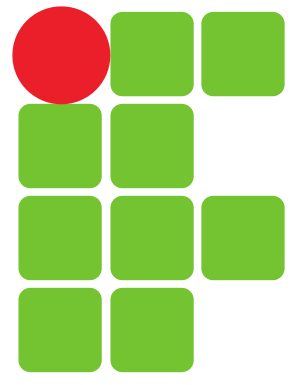
\includegraphics[scale=0.25]{figuras/logo_iff}}
    \caption{Logotipo do Instituto Federal Fluminense.}
    \label{img:logo_iff}
\end{figure}

\begin{figure}[H]
	\centering
	\subfigure[Logotipo parcialmente binarizado.]{
		
\includegraphics[scale=0.25]{figuras/logo_parcial_bin}
		\label{img:logo_parcial_bin}
	}\hspace{3em}
	\subfigure[Logotipo totalmente binarizado.]{
		
\includegraphics[scale=0.25]{figuras/logo_bin}
		\label{img:logo_bin}
	}
	\caption{Limiarização com diferentes \textit{thresholds} no logotipo do IFF.}
	\label{img:threshold_logotipo}
\end{figure}

Realizada a etapa de \textit{threshold}, pode-se então recuperar os contornos dos elementos em preto na imagem. Aplicando o método \textit{findContours()}, descrito na linha 4 do Código \ref{code:contours}, é retornada uma lista com os limites de todos os elementos. Através do Código \ref{code:num_elem}, é possível ver o comando utilizado para saber a quantidade de elementos que o OpenCV recuperou.

\begin{code}{python}{Comando para imprimir saída, contendo o número de elementos da figura.}{code:num_elem}
print len(contours)
\end{code}

Como o exemplo utiliza uma imagem binarizada com todos os objetos da imagem, o resultado é dez, representando a quantidade de elementos do \textit{array}. Apesar de haver dez elementos em preto identificáveis, a ferramenta uniu dois deles, e obteve o contorno do fundo branco, como é possível ver na Figura \ref{img:track_um_threshold}, após os contornos serem desenhados. Entretanto, pelo fato dos elementos unidos serem de cores diferentes, é possível separá-los, aplicando dois \textit{thresholds} em momentos diferentes do código. Realizada a etapa de recuperação dos contornos, os mesmos são desenhados na imagem. O resultado final é exposto na Figura \ref{img:track_dois_threshold}, enquanto o Código \ref{code:completo} contém todas as operações necessárias para se chegar a este resultado.

\begin{figure}[H]
	\centering
	\subfigure[Contornos obtidos com um \textit{threshold}.]{
		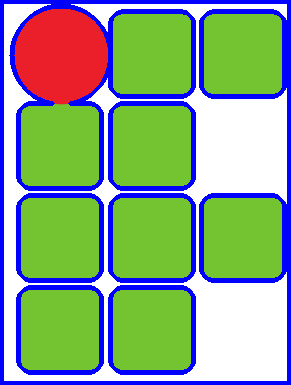
\includegraphics[scale=0.25]{figuras/track_um_threshold}
		\label{img:track_um_threshold}
	}\hspace{3em}
	\subfigure[Contornos obtidos com dois \textit{thresholds}.]{
		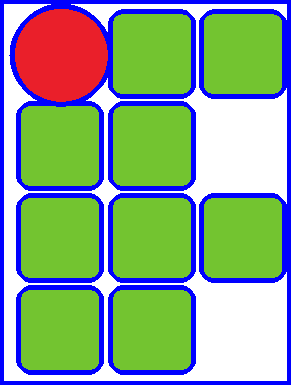
\includegraphics[scale=0.25]{figuras/track_dois_threshold}
		\label{img:track_dois_threshold}
	}
	\caption{Contornos desenhados em seus respectivos elementos. Nos contornos da Figura \ref{img:track_um_threshold}, os dados foram obtidos com apenas um \textit{threshold}, já na Figura \ref{img:track_dois_threshold} foram usados dois \textit{thresholds}.}
	\label{img:threshold_logotipo}
\end{figure}

\begin{code}{python}{Toda a lógica para obtenção dos contornos e desenho dos mesmos.}{code:completo}
img = cv2.imread('DIR_PROJETO/images/logo_iff.png')
img_gray = cv2.cvtColor(img, cv2.COLOR_BGR2GRAY)
ret, thresh_ball = cv2.threshold(img_gray, 93, 255, cv2.THRESH_BINARY)
contours, hierarchy = cv2.findContours(thresh_ball, cv2.RETR_TREE, cv2.CHAIN_APPROX_NONE)
cv2.drawContours(img, contours[1], -1, (255,0,0),3)
ret, thresh_squares = cv2.threshold(img_gray, 155, 255, cv2.THRESH_BINARY)
contours2, hierarchy = cv2.findContours(thresh_squares, cv2.RETR_TREE, \
	cv2.CHAIN_APPROX_NONE)
cv2.drawContours(img, contours2, -1, (255,0,0),3)
cv2.imwrite('DIR_PROJETO/images/saida.png', img)
\end{code}

Ainda, através dos contornos, é possível recuperar os momentos da imagem. A biblioteca realiza essa tarefa através da função \textit{moments()}. O Código \ref{code:moments} recupera os momentos do segundo contorno da lista, que contém o círculo vermelho do logotipo. Esse método retorna um dicionário, que é um tipo de dados da linguagem Python. Ao exibir as informações contidas nessa lista, é possível visualizar todos os pares de chave e valor do dicionário (Código \ref{code:saida_moments}).

\begin{code}{python}{Os momentos são recuperados ao passar um contorno que representa um objeto da imagem.}{code:moments}
moments = cv2.moments(contours[1])
\end{code}

\begin{code}{python}{Os valores dos momentos do segundo elemento do logotipo do IFF são mantidos por um dicionário, um tipo de dados do Python.}{code:saida_moments}
{'mu02': 4466250.579995997, 'mu03': 2.099651949538806e-06, 'm11': 24999544.25,
 'nu02': 0.07959091389346826, 'm12': 1642430867.25, 'mu21': -6560.77209803462,
 'mu20': 4465517.828794554, 'nu20': 0.07957785588502587, 'm30': 2505168506.5,
 'nu21': -1.350844812113205e-06, 'mu11': -4485.94523428008,
 'mu12': -19483.180956840515, 'nu11': -7.994188290096345e-05,
 'nu12': -4.011533021684291e-06, 'm02': 26989947.0, 'm03': 1969781748.75,
 'm00': 7491.0, 'm01': 410761.5, 'mu30': 23255.18666744232,
 'nu30': 4.788178555058973e-06, 'm10': 455995.0, 'm20': 32223018.833333332,
 'm21': 1766364339.4166667}
\end{code}

Essas chaves são de três tipos: \textit{mu} (momentos centrais), \textit{nu} (momentos centrais normalizados) e \textit{m} (momentos espaciais). Ainda existem os momentos invariantes, também conhecidos como momentos \textit{Hu}, que podem ser recuperados através do método \textit{HuMoments()}. Mais sobre momentos no OpenCV podem ser encontrados no trabalho realizado por \citeonline{KILIAN}.

Através desses momentos, é possível obter características dos objetos, como sua área e centróide. A área do objeto é contida na chave \textit{m00}. Tendo esse valor, encontra-se então as coordenadas x e y do centro de massa do objeto (Código \ref{code:param_moments}).

\begin{code}{python}{Operações com os momentos do segundo elemento da lista de contornos.}{code:param_moments}
area = moments['m00']
x = moments['m10'] / area
y = moments['m01'] / area
\end{code}

Caso esteja definido a forma do objeto a ser encontrado, como um círculo, se torna interessante a recuperação de outros dados específicos dessa forma. Com isso, o resultado final tende a ser mais preciso, devido ao aumento de informações recuperadas do objeto a ser detectado. Como no exemplo apresentado é utilizado um objeto em forma circular, uma das informações relevantes a ser recuperada a respeito desse objeto é o seu raio. Isso é feito usando a fórmula da geometria, junto ao valor da área do contorno. Então, desenhando os valores encontrados, determina-se exatamente o centro e contorno do círculo vermelho em relação a figura em que ele está inserido (Código \ref{code:draw_circle}). O resultado é exposto na Figura \ref{img:track_final}.

\begin{code}{python}{Desenho feito na imagem de exemplo usando os parâmetros calculados a partir do momentos do contorno.}{code:draw_circle}
raio = sqrt(area/3.14)
cv2.circle(img, (int(x),int(y)), int(raio), (255,0,0), 3)
cv2.circle(img, (int(x),int(y)), 3, (255,0,0), -1)
\end{code}

\begin{figure}[H]
    \centering
    {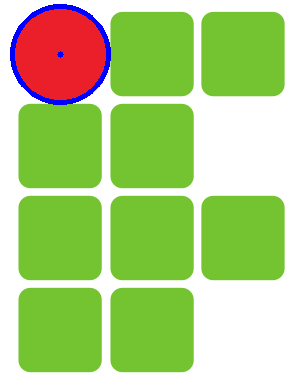
\includegraphics[scale=0.25]{figuras/track_final}}
    \caption{Rastreamento feito no círculo vermelho do logotipo do IFF.}
    \label{img:track_final}
\end{figure}

A biblioteca ainda conta com recursos para manipulações com vídeo, onde pode-se utilizar arquivos de vídeo ou câmeras, como a de um notebook. Para o caso de uma câmera de um nootebook usa-se o comando mostrado no Código \ref{code:video_opencv}.\newline\newline

\begin{code}{python}{Inicialização do vídeo através da biblioteca OpenCV.}{code:video_opencv}
video = cv2.VideoCapture(0)
\end{code}

Um número inteiro é passado pela função que recupera o vídeo, representando o identificador do dispositivo de vídeo. A partir desse objeto, cria-se então uma rotina para captura e apresentação dos \textit{frames} do vídeo em uma nova janela (Código \ref{code:loop_video}).

\begin{code}{python}{Lógica para processamento e visualização dos \textit{frames} do vídeo.}{code:loop_video}
while video.grab():
	flag, frame = video.retrieve()
	if flag:
		cv2.imshow('Video', frame)
		cv2.waitKey(1)
\end{code}

Tendo em mente que um vídeo é composto por diversas imagens em sequência, os mesmos tratamentos feitos em imagens também podem ser utilizados em vídeos, como aplicação de filtros e desenhos. Isso abrange as possibilidades em inúmeras atividades, que podem evoluir até sistemas completos de Visão Computacional.

\section{SimpleCV}

SimpleCV\footnote{\url{http://simplecv.org}} é um \textit{framework}\footnote{Coleção abstrata de classes, interfaces e padrões dedicados a resolver um conjunto de problemas através de uma arquitetura flexível e extensível.} de código aberto que foi desenvolvido pelos engenheiros da Sight Machine, e está sob a licença BSD (\textit{Berkeley Software Distribution}). O \textit{framework} é portável nas plataformas Mac, Windows e distribuições Linux Ubuntu e Arch Linux.

O objetivo do \textit{framework} é tornar mais fácil aos programadores o desenvolvimento de sistemas de Visão Computacional, simplificando muitas das tarefas mais comuns. \citeonline{DEMAAGD} destacam que, por ser uma biblioteca simples, não é necessário possuir muitos conhecimentos em Python e especialização na área da computação, sendo preciso apenas o interesse em Visão Computacional.

\subsection{Estrutura}

Em sua implementação, o SimpleCV utiliza bibliotecas existentes para Python na área de Visão Computacional, reunindo os recursos mais importantes de cada uma delas. A Figura \ref{img:estrutura_simplecv} expõe a relação do SimpleCV com as bibliotecas existentes no mercado. É destacado pelo diagrama a nova camada criada pelo SimpleCV, que acessa os recursos necessários das bibliotecas para Python. Dessa forma, grande parte das tarefas de Visão Computacional comumente realizadas, tornam-se mais simples.

\begin{figure}[h]
    \centering
	{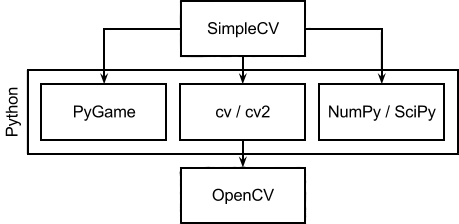
\includegraphics[scale=0.75]{figuras/estrutura_simplecv}}
    \caption{Bibliotecas usadas pelo SimpleCV divididas em camadas.}
    \label{img:estrutura_simplecv}
\end{figure}

Segundo sua documentação oficial\footnote{\url{http://simplecv.org/docs}}, o SimpleCV se encontra em sua versão 1.3 dividido em conjuntos de classes. Essa classes são separadas da seguinte forma: \textit{Features}, \textit{MachineLearning}, \textit{Segmentation} e \textit{Shell}. O pacote \textit{Features}, conta com métodos para classificação de objetos em imagens, baseando-se em suas características. O conjunto de classes contidos no pacote \textit{MachineLearning} implementam alguns algoritmos de classificação, como o \textit{k-nearest neighbor} e \textit{Naive Bayes}. O pacote \textit{Segmentation} contém classes para segmentação de imagens, podendo ser diferenciada por cor ou comparando diferenças entre dois \textit{frames}. A classe \textit{Shell} permite que a biblioteca seja usada via terminal, tendo dessa forma, resposta rápida para dúvidas que surgirem durante o desenvolvimento, realização de testes rápidos e acesso a última documentação dos objetos do SimpleCV. Essa implementação é baseada no IPython.

Além desses pacotes, existem ainda as classes básicas da ferramenta, sendo elas: \textit{Camera}, \textit{Color}, \textit{ColorModel}, \textit{Display}, \textit{DrawingLayer}, \textit{EXIF}, \textit{Font}, \textit{ImageClass} e \textit{Stream}. Cada uma delas possui uma finalidade distinta. Com a classe \textit{Camera}, por exemplo, é possível trabalhar com vídeo de diversos dispositivos, como a de um notebook, de câmeras que enviam sinais pela Internet (\textit{stream}) ou até mesmo da câmera do Kinect\footnote{Sensor de movimentos de última geração, desenvolvimento inicialmente para jogos eletrônicos.}, dispositivo desenvolvido pela Microsoft. Outras classes fornecem manipulações com interface, mostrando resultados de imagens e vídeo em janelas do sistema operacional e eventos com o mouse, e desenhos básicos de formas e texto.

\subsection{Instalação}

Existem diversas formas de realizar a instalação do SimpleCV no Linux Ubuntu 11.10. Independente do método escolhido para a instalação do \textit{framework}, existem dependências que precisam ser instaladas previamente. São elas: Python (2.7 ou superior), Python Setup Tools, PyGame, NumPy, SciPy, Easy Install e o OpenCV. Essas dependências podem ser instaladas através do comando mostrado no Código \ref{code:depend_simplecv}.

\begin{terminal}{Instalação das dependências do SimpleCV.}{code:depend_simplecv}
sudo apt-get install python-setuptools python-pygame python-scipy
\end{terminal}

Por padrão as dependências restantes já vem instaladas na versão 11.10 do Linux Ubuntu, sendo um caso isolado o OpenCV, que possui um processo de instalação, como mostrado na Seção \ref{section:install_opencv}. Para a instalação do SimpleCV em si, é necessário realizar o download do pacote .deb em seu site oficial\footnote{\url{http://simplecv.org/download}}. Caso esteja tudo devidamente configurado, basta executar o .deb e a instalação será feita. No entanto, nos testes realizados, essa instalação apresentou problemas ao executar um \textit{script} simples de uso da ferramenta. Como solução, foi necessário baixar a última versão da biblioteca do repositório de controle de versão do projeto, o GitHub. Realizada esta operação, bastou entrar na pasta que foi criada e executar o arquivo de instalação, utilizando o próprio interpretador do Python. Essas operações são mostradas no Código \ref{code:install_simplecv_git}, que inclui a instalação do Git, necessário para realizar o download do código fonte do repositório de controle de versão.

\begin{terminal}{Instalação da biblioteca SimpleCV através do GitHub.}{code:install_simplecv_git}
sudo apt-get install git
git clone git://github.com/ingenuitas/SimpleCV.git SimpleCV
sudo apt-get install python-setuptools
sudo python setup.py install
\end{terminal}

Além de possuir bibliotecas essenciais para o seu funcionamento, o SimpleCV também conta com algumas bibliotecas opcionais para uso exclusivo em determinados projetos, como PIP, BeautifulSoup, webm, freenect, entre outros.

Também é possível fazer com que o SimpleCV seja utilizado em interatividade com o shell. Para isso, é necessário a instalação do IPython, uma ferramenta da linguagem Python para shell. O download dessa ferramenta pode ser feito pelo seu site\footnote{\url{http://ipython.org}}, ou ser baixada e instalada automaticamente através do terminal (Código \ref{code:install_ipython}).

\begin{terminal}{Instalação do IPython.}{code:install_ipython}
sudo apt-get install ipython
\end{terminal}

\subsection{Uso prático}

Para modo comparativo, serão mostradas nesta Seção funções equivalentes às utilizadas na Seção sobre OpenCV.

Diferente da interface \textit{cv2} do OpenCV, o \textit{framework} SimpleCV conta com classes próprias para manipulação de imagens, assemelhando-se a interface \textit{cv2.cv}. Ao ler sua documentação, percebe-se que a proposta da ferramenta é facilitar o trabalho do programador, evitando que manipulações manuais sejam feitas. Neste caso, por possuir a maioria das operações necessárias, o uso do \textit{framework} evita trabalhos repetitivos normalmente realizados no desenvolvimento de sistemas de Visão Computacional. Por outro lado, essa filosofia de uso da ferramenta torna o aprendizado um pouco lento, sendo necessário constantes consultas a descrições de métodos e estruturas de dados em sua documentação.

A seguir, são mostrados exemplos de operações que podem ser feitas com a ferramenta. Como exemplo inicial, é exposto no Código \ref{code:img_simplecv} o carregamento de uma imagem utilizando o \textit{framework} SimpleCV.

\begin{code}{python}{Carregamento de uma imagem utilizando o \textit{framework} SimpleCV.}{code:img_simplecv}
from SimpleCV import Image
img = Image('DIR_PROJETO/images/logo_iff.png')
\end{code}

A imagem carregada é criada como uma classe do próprio \textit{framework}, \textit{SimpleCV.Image}. Nela, estão implementadas diversas funções para ações que podem ser feitas com a imagem, como mostrá-la na tela ou acessar seus \textit{pixels}. Para acessar um pixel da imagem, por exemplo, utiliza-se o método \textit{getPixel()}. Caso opte-se por manipular manualmente seus \textit{pixels}, é possível recuperar o mesmo tipo de objeto retornado por padrão pela interface \textit{cv2} do OpenCV, através do método \textit{getNumpy()}.

Seguindo a mesma ideia, outras manipulações podem ser realizadas, como transformar uma imagem em binária, alterar seu espaço de cor ou aplicar filtros (Código \ref{code:convert_img}).

\begin{code}{python}{Conversões de espaço de cor utilizando a ferramenta SimpleCV.}{code:convert_img}
# Binarizacao em preto e branco
img.binarize()
# Binarizacao em branco e preto
img.binarize().invert()

# Conversao para RGB
img.toBGR()
# Conversao para HSV
img.toHSV()
# Conversao para escala de cinza
img.toGray()

# Aplicacao do filtro dilatar
img.dilate()
# Aplicacao do filtro corroer
img.erode()
\end{code}

O método \textit{binarize()} aplica um limiar na imagem, tornando os valores acima desse limiar em preto, e os valores abaixo em branco. Ao utilizar o método \textit{invert()}, esses valores são invertidos. O método \textit{threshold()} também pode ser utilizado para se ter o mesmo resultado, contudo, por padrão são colocados os \textit{pixels} abaixo desse limiar em preto, e os acima em branco. Pode-se também passar valores como parâmetros para determinar este limiar.

Quanto as transformações nos espaços de cores da imagem usados no exemplo acima, os métodos utilizados são bastante intuitivos. O método \textit{toBGR()} transforma os valores dos \textit{pixels} da imagem seguindo a ordem azul, verde e vermelho, mesmo padrão utilizado pelo OpenCV. Já o método \textit{toHSV()} realiza essa transformação para os componentes matiz, saturação e valor. Ainda, o método \textit{toGray()} transforma a imagem para escala de cinza.

Por fim, os filtros utilizados no exemplo são filtros morfológicos que alteram a forma dos objetos na imagem. Através do método \textit{dilate()}, os limites dos objetos com mais brilho são expandidos, e os que são mais escuros reduzidos. No método \textit{erode()} ocorre o inverso, os limites dos objetos com mais brilho são reduzidos, e os mais escuros são expandidos.

Com os recursos disponibilizados pelo \textit{framework}, também é possível a recuperação de \textit{blobs}\footnote{Ponto ou uma região na imagem que difere em propriedades como brilho ou cor se comparado ao ambiente a sua volta.} através de máscaras, que são imagens binárias possuindo apenas a região de interesse a ser detectada em branco, e o resto em preto \cite{RAHMAN}. A máscara passada como no exemplo exposto no Código \ref{code:blobs_simplecv}, deve possuir as mesmas dimensões da imagem original, além de ser necessário ter sido passada previamente por uma etapa de processamento, como utilização de métodos como \textit{binarize()} ou \textit{toGray()}. Esses \textit{blobs}, então são desenhados usando o método \textit{draw()}, tendo ainda a possibilidade de passagem de parâmetros para determinar a cor e o tamanho da linha a ser desenhada.

\begin{code}{python}{Recuperação dos \textit{blobs} são feitos através da imagem, enquanto o responsável por desenhá-los é objeto \textit{blob}.}{code:blobs_simplecv}
from SimpleCV import Color
blobs = img.findBlobsFromMask(img.binarize(155))
blobs.draw(Color.BLUE, 3)
\end{code}

Por sua vez, os momentos podem ser acessados após a recuperação dos \textit{blobs} da imagem. Ao utilizar o método \textit{findBlobsFromMask()}, é retornado um \textit{FeatureSet} contendo todos os \textit{blobs} da imagem, com base na máscara passada. Ao executar o método \textit{show()}, esses \textit{blobs} são contornados. Ainda, pode-se acessar cada momento em particular, simplesmente chamando a variável de um \textit{blob} no vetor em que está contido. Essas operações podem ser melhor entendidas através do Código \ref{code:moments_simplecv}.

\begin{code}{python}{Operações com momentos dos \textit{blobs} com o \textit{framework} SimpleCV.}{code:moments_simplecv}
# Visualizando todos os blobs
blobs.show()

# Visualizando o blob na posicao 8 do vetor
blobs[8].show()

# Acessando os momentos do blob na posicao 0 do vetor
blobs[0].m00
blobs[0].m10
blobs[0].m01
\end{code}

Assim como o OpenCV, o SimpleCV suporta diversos dispositivos de câmera diferentes. Para habilitar essa funcionalidade no \textit{framework}, são utilizados os comandos no Código \ref{code:video_simplecv}. As linhas do exemplo mostram como inicializar uma câmera local, podendo ser utilizada  uma embutida em um notebook ou uma instalada no próprio computador pessoal, através, por exemplo, de uma conexão USB.\newline\newline\newline\newline


\begin{code}{python}{Lógica para inicialização de vídeo com o \textit{framework} SimpleCV.}{code:video_simplecv}
from SimpleCV import Camera
cam = Camera()
while True:
	cam.getImage().show()
\end{code}

\section{Conclusão}

Apesar de haver diversas bibliotecas para auxiliar o desenvolvimento de sistemas de Visão Computacional, existe apenas um conjunto limitado com suporte para linguagem Python. Nas pesquisas realizadas, a biblioteca OpenCV se mostrou predominante em se tratando de ferramentas para uso geral. Assuntos relacionados a ferramenta são facilmente encontrados, facilitando a aproximação dos iniciantes da área de Visão Computacional com a biblioteca. Sua documentação também é bastante detalhada, onde são mostrados exemplos de uso da maioria das funções disponíveis.

Em se tratando do suporte para linguagem Python, as diferenças entre as interfaces do OpenCV disponíveis não são claramente apresentadas. No trabalho realizado, o impacto dessa falta de clareza atrasou o desenvolvimento do estudo de caso. Os estudos foram iniciados utilizando a interface \textit{cv} e, percebendo a existência e vantagens da interface \textit{cv2}, mudou-se o foco nas pesquisas.

Complementando os estudos, o \textit{framework} SimpleCV mostrou-se promissor. A ferramenta reúne diversos recursos comumente utilizados, minimizando o esforço repetitivo no desenvolvimento de sistemas de Visão Computacional. Percebe-se que o \textit{framework} não foi criado para substituir o OpenCV, pelo contrário, é uma ferramenta complementar que pode ser utilizada em conjunto com o OpenCV, caso esse seja o desejo do desenvolvedor.

\citeonline{OLIVER} descreve um comparativo entre a biblioteca OpenCV e o \textit{framework} SimpleCV levando em conta diversos aspectos: facilidade no uso, velocidade, recursos necessários para execução, custo, ambiente de desenvolvimento, gerenciamento de memória, portabilidade, entre outros. Nos quesitos facilidade no uso e gerenciamento de memória, o SimpleCV se mostra bastante superior em comparação com o OpenCV. Por outro lado, nos quesitos velocidade e portabilidade, o OpenCV se torna uma melhor opção.

Na perspectiva de iniciantes da área de Visão Computacional, que desconhecem quaisquer ferramentas disponíveis para uso no desenvolvimento de aplicações, o acervo de materiais encontrados na Internet são em sua grande maioria voltado para o OpenCV. Conclui-se, então, que apesar do \textit{framework} SimpleCV facilitar o processo de desenvolvimento em diversos aspectos, o OpenCV proporciona uma curva de aprendizado melhor, por trazer na literatura assuntos práticos relacionados ao desenvolvimento de sistemas de Visão Computacional.

Com base nisso, utilizou-se a biblioteca OpenCV em conjunto com a interface \textit{cv2} para Python para desenvolvimento da aplicação apresentada como estudo de caso deste trabalho.
